\documentclass{article}

\usepackage{postprocess/context/arxiv}

\usepackage[utf8]{inputenc} % allow utf-8 input
\usepackage{amsmath}
\usepackage[T1]{fontenc}    % use 8-bit T1 fonts
\usepackage{hyperref}       % hyperlinks
\usepackage{url}            % simple URL typesetting
\usepackage{booktabs}       % professional-quality tables
\usepackage{amsfonts}       % blackboard math symbols
\usepackage{nicefrac}       % compact symbols for 1/2, etc.
\usepackage{microtype}      % microtypography
\usepackage{graphicx}
\usepackage{natbib}
\usepackage{doi}
\usepackage{float}
\usepackage{subcaption}
\usepackage{wrapfig}

\title{Causal Discovery Report on Abalone}

\author{ \href{https://orcid.org/0000-0000-0000-0000}{
\includegraphics[scale=0.06]{postprocess/context/orcid.pdf}\hspace{1mm}Causal Copilot}}

\renewcommand{\headeright}{Technical Report}
\renewcommand{\undertitle}{Technical Report}

\hypersetup{
pdftitle={Causal Discovery Report on Abalone},
pdfauthor={Causal Copilot},
pdfkeywords={Causal Discovery, Large Language Model, PC, Abalone},
}

\begin{document}
\maketitle

\begin{abstract}
This study conducts a causal discovery analysis on a dataset of abalones, focusing on critical variables such as age, shell measurements, and internal organ weights. Utilizing a comprehensive methodology, we first preprocessed the data to ensure its quality and then employed a large language model to inform the selection of suitable causal discovery algorithms, including the PC, GES, and NOTEARS algorithms, justified by the dataset's characteristics. The resultant causal relationships reveal nuanced interactions among biological metrics, with age significantly influencing various growth and structural features. Our findings delineate a complex hierarchy of growth interdependencies, highlighting age's prominent role in shaping the dimensions and weights of abalones. This research contributes to the understanding of abalone biology and provides a foundation for future conservation efforts, emphasizing the need for careful interpretation of statistical relationships, particularly where expert knowledge overlaps with causal inference.
\end{abstract}

\keywords{Causal Discovery, Large Language Model, PC, Abalone}

\raggedbottom
\section{Introduction}
Causal discovery in datasets concerning marine organisms, such as abalones, is pivotal for unraveling the intricate relationships among various biological metrics that reflect their growth, health, and reproductive status. The dataset at hand includes several key variables, including age, shell measurements (length, diameter, height, and weight), and internal organ weights, all of which are interrelated. As abalones age, they typically grow larger, which affects their overall weight and structural characteristics. Understanding these dependencies is crucial not only for enhancing our knowledge of abalone biology but also for informing sustainable management practices in marine ecosystems. By leveraging insights from marine biology, including growth patterns, reproductive cycles, and ecological interactions, this report aims to uncover causal relationships within the dataset, potentially guiding future research and conservation efforts.

\section{Background Knowledge}
\subsection{Detailed Explanation about the Variables}
\begin{itemize}
\item \textbf{Age}: This variable likely represents the age of the abalones, which is typically determined by counting the number of rings on their shells. Age is a significant factor in the study of growth patterns, reproductive status, and overall life history traits of abalones.
\item \textbf{Length}: This variable refers to the longest shell measurement of the abalone, providing a quantitative assessment of size that is crucial for understanding growth dynamics and biological fitness.
\item \textbf{Shell Weight}: This represents the weight of the shell itself. It serves as an important indicator of the structural integrity and physical condition of the abalone and can be associated with age and growth rates.
\item \textbf{Diameter}: This measurement usually captures the distance across the shell at its widest point. Like length, diameter contributes to characterizing the overall size of the abalone and can indicate developmental health.
\item \textbf{Height}: This variable measures the vertical dimension of the abalone's shell. Alongside length and diameter, height plays a vital role in completing the morphological profile of the abalone.
\item \textbf{Whole Weight}: This is the total weight of the abalone, including both the shell and the flesh. Whole weight is an essential metric for assessing the overall size, health, and market value of the abalone.
\item \textbf{Shucked Weight}: This variable indicates the weight of the edible flesh after the shell has been removed. It is a key measurement for evaluating the market value and quality yield of the abalone.
\item \textbf{Viscera Weight}: This measures the weight of the internal organs of the abalone. It can be indicative of both health status and reproductive development, providing insight into the organism's biological condition. 
\end{itemize}

Understanding these variables is fundamental for analyzing the growth, health, and ecological interactions of abalones, facilitating more informed causal discovery analyses in this dataset.

\subsection{Possible Causal Relations among these Variables}
\begin{minipage}[t]{0.7\linewidth}
\begin{itemize}
    \item \textbf{Age $\rightarrow$ Length}: As abalones age, they tend to grow larger, hence older abalones are generally longer.
    \item \textbf{Age $\rightarrow$ Diameter}: Similar to length, the age of an abalone is likely to influence its diameter, with older individuals having a larger diameter.
    \item \textbf{Age $\rightarrow$ Height}: The height of the abalone is expected to increase with age, reflecting overall growth patterns as abalones mature.
    \item \textbf{Length $\rightarrow$ Whole Weight}: There is a strong likelihood that as the length of an abalone increases, its whole weight will also increase due to the additional biomass.
    \item \textbf{Diameter $\rightarrow$ Whole Weight}: An increase in diameter is likely to correlate with increases in whole weight, as the overall size of the abalone contributes to its mass.
    \item \textbf{Height $\rightarrow$ Whole Weight}: Similar to length and diameter, an increase in height usually implies an increase in the whole weight of the abalone.
    \item \textbf{Whole Weight $\rightarrow$ Shucked Weight}: The total weight of the abalone (whole weight) causally affects shucked weight, as the weight of the edible flesh is a component of the whole.
    \item \textbf{Whole Weight $\rightarrow$ Viscera Weight}: Whole weight also causally relates to viscera weight, since the internal organs contribute to the overall mass of the abalone.
    \item \textbf{Shell Weight $\rightarrow$ Diameter}: As the diameter of the abalone increases, it is likely that the shell weight will also increase, reflecting a larger shell.
    \item \textbf{Length $\rightarrow$ Shell Weight}: The length of the abalone can also influence shell weight; longer abalones generally have heavier shells.
    \item \textbf{Diameter $\rightarrow$ Shell Weight}: An increase in the diameter of the abalone likely leads to a corresponding increase in shell weight, again reflecting its relationship to size.
    \item \textbf{Height $\rightarrow$ Shell Weight}: Similar to the other dimensions, height may also have a positive influence on shell weight, as taller abalones typically have more substantial shells.
\end{itemize}
\end{minipage}
\hspace{0.05\textwidth}
\begin{minipage}[t]{0.3\linewidth}
    \begin{figure}[H]
        \centering
        \resizebox{\linewidth}{!}{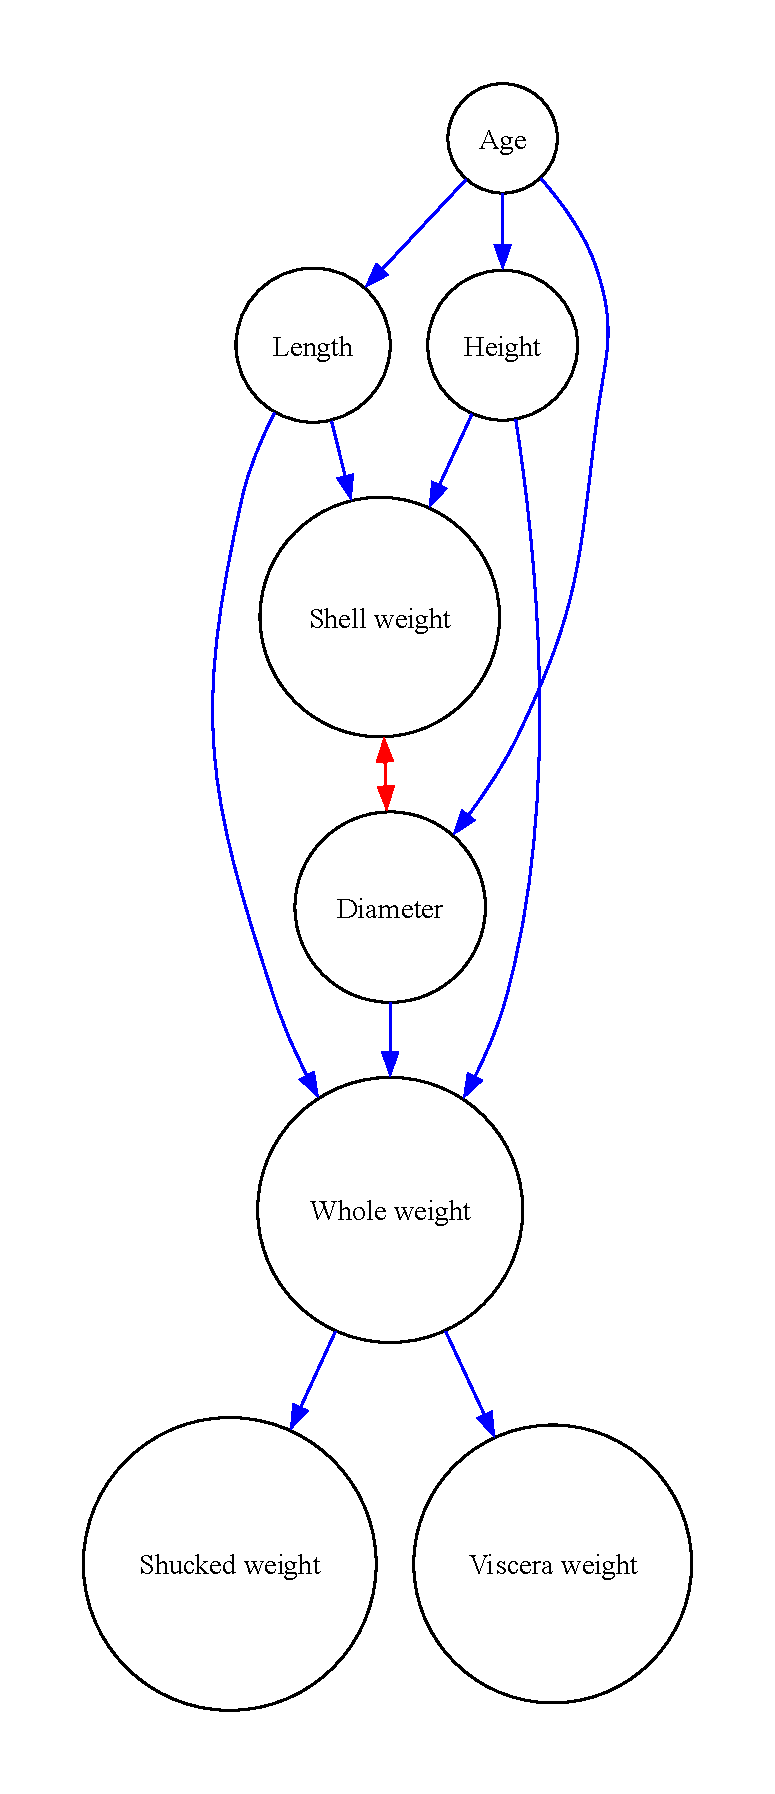
\includegraphics[height=0.4\textheight]{./demo_data/20241104_114158/Abalone/output_graph/potential_relation.pdf}}
        \caption{\label{fig:relation}Possible Causal Relation Graph}
    \end{figure}
\end{minipage}

\section{Dataset Descriptions and EDA}
The following is a preview of our original dataset.

\begin{table}[H]
    \centering
    \caption{Dataset Preview}
    \begin{tabular}{rrrrrrrr}
\toprule
 Age &  Length &  Shell weight &  Diameter &  Height &  Whole weight &  Shucked weight &  Viscera weight \\
\midrule
15.0 &   0.455 &         0.365 &     0.095 &  0.5140 &        0.2245 &          0.1010 &           0.150 \\
 7.0 &   0.350 &         0.265 &     0.090 &  0.2255 &        0.0995 &          0.0485 &           0.070 \\
 9.0 &   0.530 &         0.420 &     0.135 &  0.6770 &        0.2565 &          0.1415 &           0.210 \\
10.0 &   0.440 &         0.365 &     0.125 &  0.5160 &        0.2155 &          0.1140 &           0.155 \\
 7.0 &   0.330 &         0.255 &     0.080 &  0.2050 &        0.0895 &          0.0395 &           0.055 \\
\bottomrule
\end{tabular}

\end{table}

\subsection{Data Properties}
We employ several statistical methods to identify data properties.

The shape of the data, data types, and missing values are assessed directly from the dataframe. Linearity is evaluated using Ramsey’s RESET test, followed by the Benjamini \& Yekutieli procedure for multiple test correction. Gaussian noise is assessed through the Shapiro-Wilk test, also applying the Benjamini \& Yekutieli procedure for multiple test correction. Time-Series and Heterogeneity are derived from user queries.

Properties of the dataset we analyzed are listed below.

\begin{table}[H]
    \centering
    \caption{Data Properties}
    \begin{tabular}{rrrrrrr}
    \toprule
    Shape ($n$ x $d$) & Data Type & Missing Value & Linearity & Gaussian Errors & Time-Series & Heterogeneity \\
    \midrule
    (4177, 8)   & Continuous & False & False & False & False & False \\
    \bottomrule
    \end{tabular}
\end{table}

\subsection{Distribution Analysis}
The following figure shows distributions of different variables. The orange dash line represents the mean, and the black line represents the median. Variables are categorized into three types according to their distribution characteristics.

\begin{figure}[H]
\centering
\includegraphics[width=\linewidth]{./demo_data/20241104_114158/Abalone/output_graph/eda_dist.jpg}
\caption{\label{fig:dist}Distribution Plots of Variables}
\end{figure}

\begin{itemize}
\item Slight left skew distributed variables: Length, Shell Weight, Diameter, Whole Weight
\item Slight right skew distributed variables: Age, Height, Shucked Weight, Viscera Weight
\item Symmetric distributed variables: None
\end{itemize}

\subsection{Correlation Analysis}
\begin{minipage}[t]{0.5\linewidth}
    In this analysis, we will categorize the correlation statistics of features in the dataset into three distinct categories: Strong correlations ($r>0.8$), Moderate correlations ($0.5<r<0.8$), and Weak correlations ($r<0.5$).

\begin{itemize}
\item Strong Correlated Variables: Shell weight and Length, Shell weight and Height, Shell weight and Viscera weight, Length and Height, Whole weight and Height, Whole weight and Shucked weight, Shucked weight and Height, Shucked weight and Shell weight, Viscera weight and Height, Viscera weight and Shell weight
\item Moderate Correlated Variables: Length and Age, Shell weight and Age, Diameter and Age, Diameter and Length, Height and Age, Diameter and Shucked weight, Whole weight and Diameter, Viscera weight and Diameter, Viscera weight and Whole weight, Whole weight and Length
\item Weak Correlated Variables: Shucked weight and Age
\end{itemize}
\vfill
\end{minipage}
\hfill
\begin{minipage}[t]{0.5\linewidth}
    \begin{figure}[H]
        \centering
        \vspace{-1.5cm}
        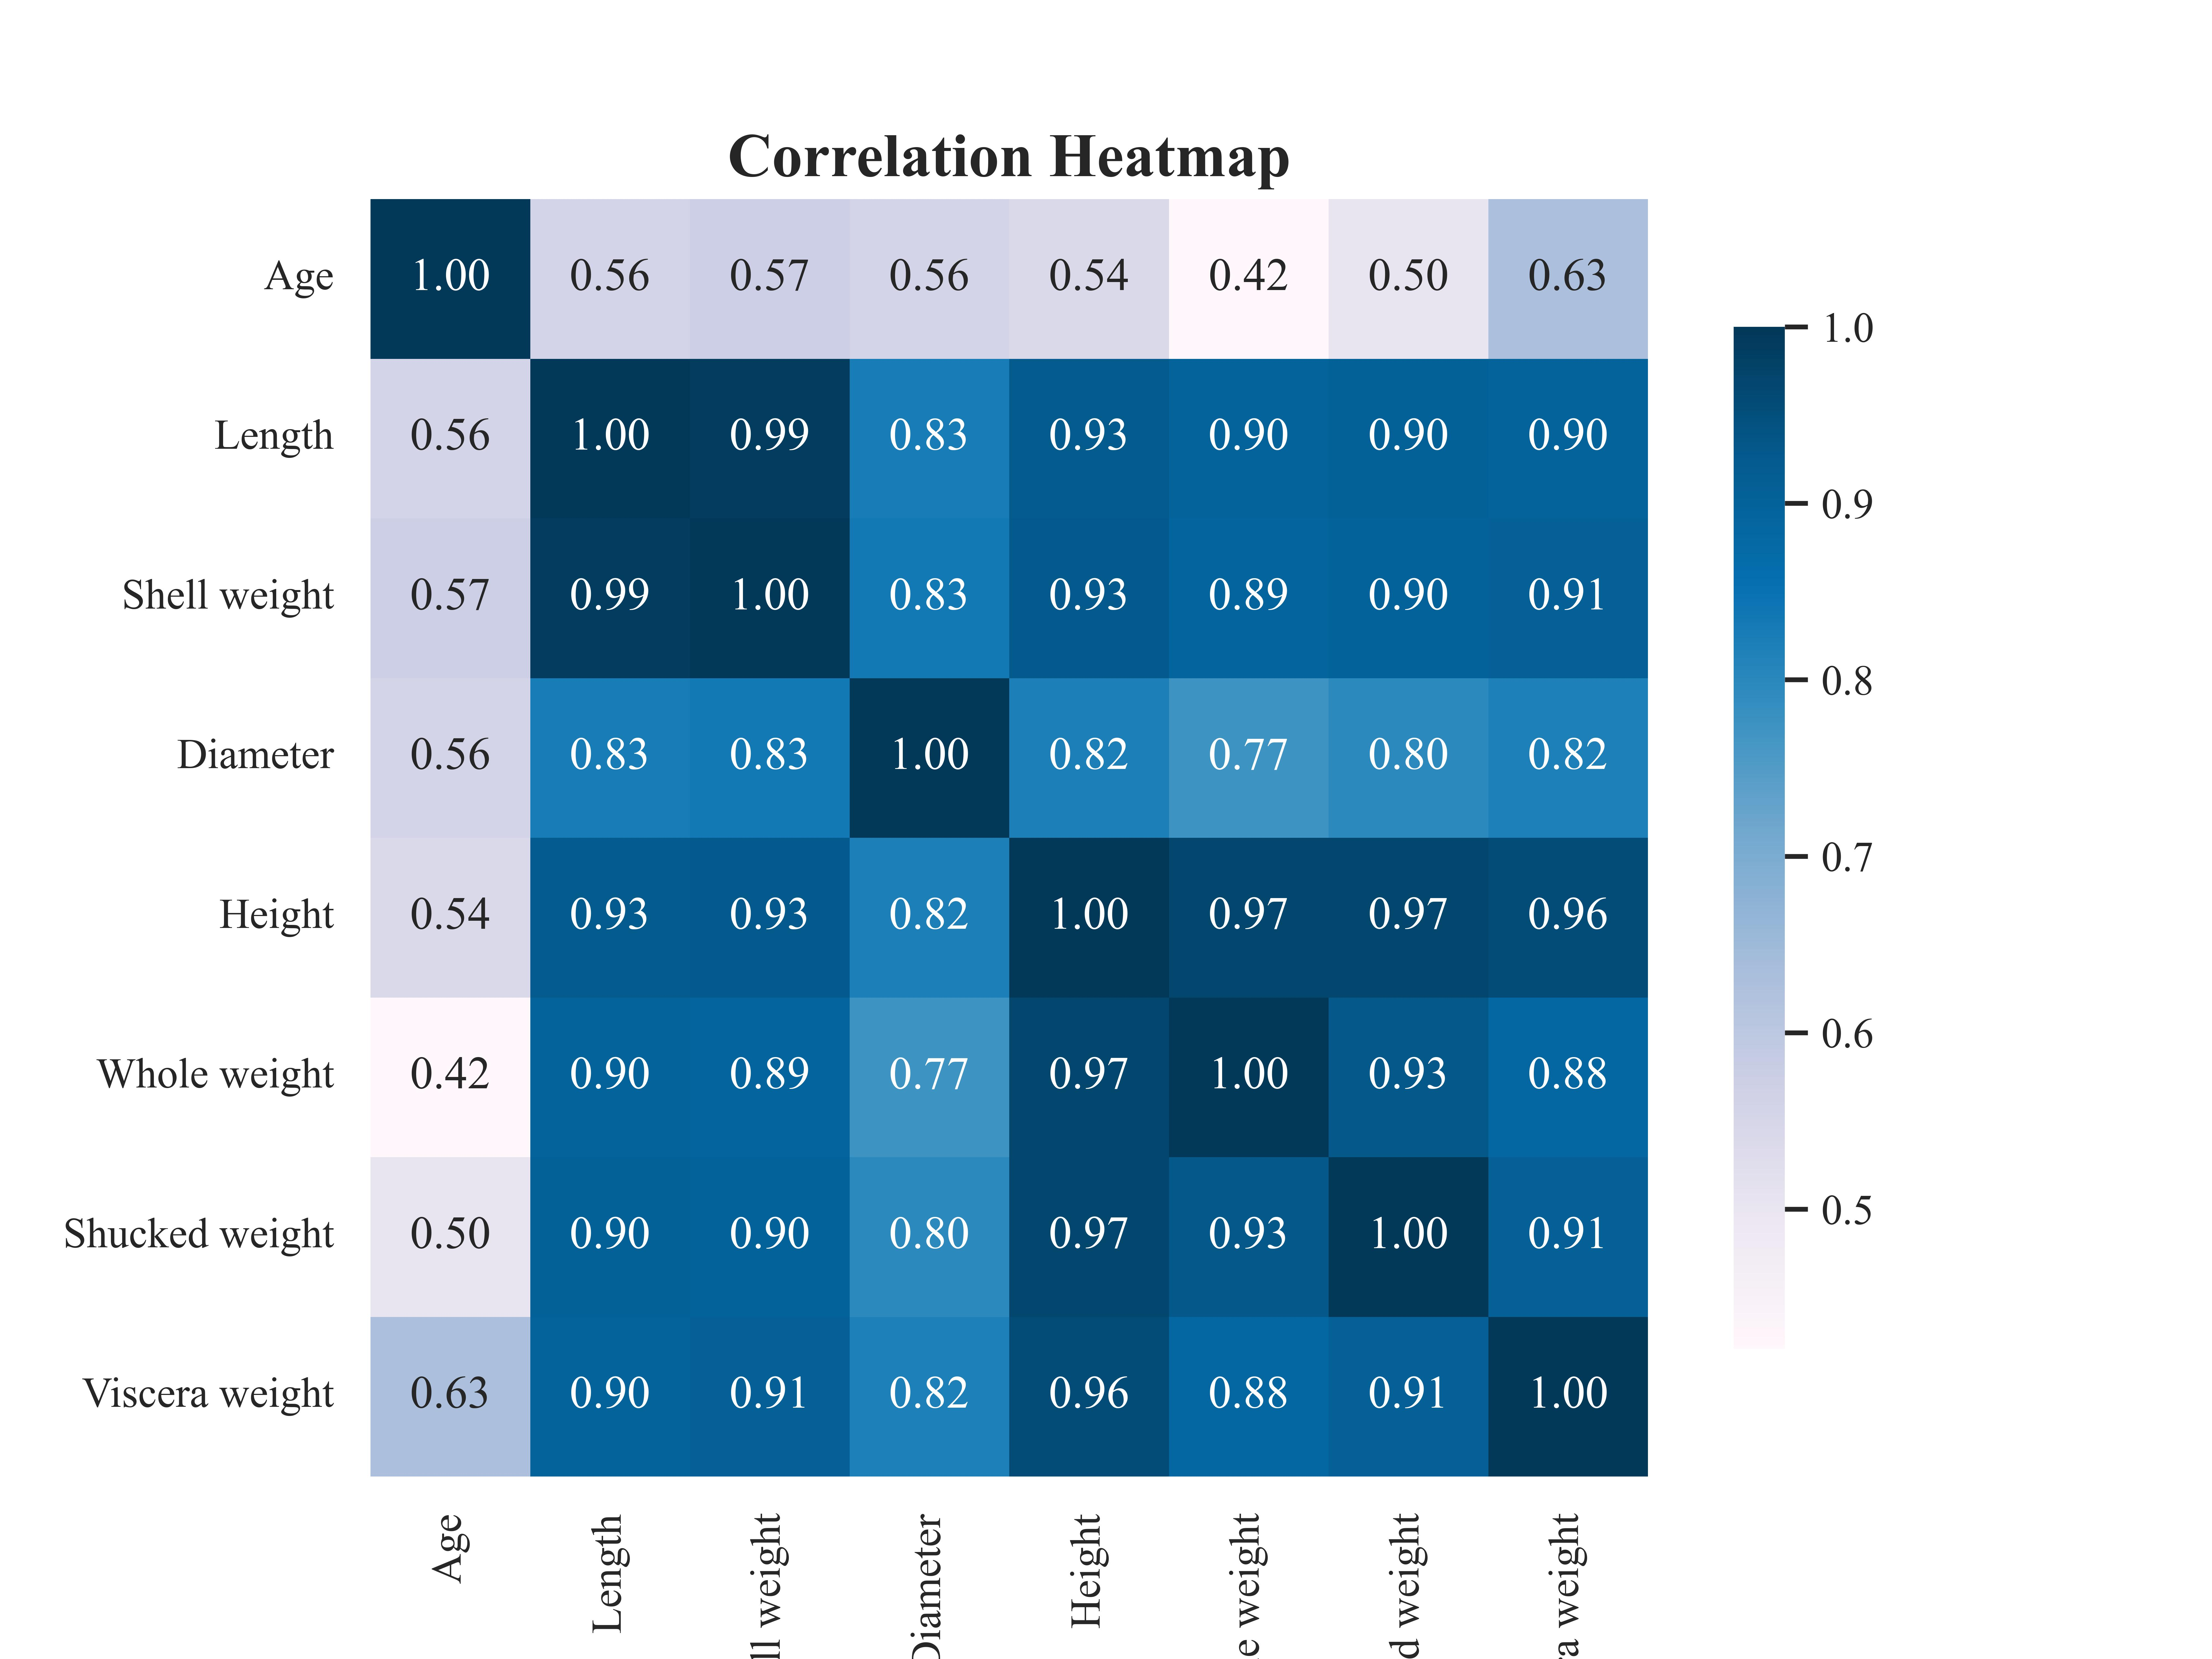
\includegraphics[width=\linewidth]{./demo_data/20241104_114158/Abalone/output_graph/eda_corr.jpg}
        \caption{\label{fig:corr}Correlation Heatmap of Variables}
    \end{figure}
\end{minipage}

\section{Discovery Procedure}
In this section, we provide a detailed description of the causal discovery process implemented by Causal Copilot. We also provide the chosen algorithms and hyperparameters, along with the justifications for these selections.

\subsection{Data Preprocessing}
In this initial step, we preprocessed the data and examined its statistical characteristics. This involved cleaning the data, handling missing values, and performing exploratory data analysis to understand distributions and relationships between variables.

\subsection{Algorithm Selection assisted with LLM}
Following data preprocessing, we employed a large language model (LLM) to assist in selecting appropriate algorithms for causal discovery based on the statistical characteristics of the dataset and relevant background knowledge. The top three chosen algorithms, listed in order of suitability, are as follows:   

\begin{itemize}
    \item \textbf{PC}:
        \begin{itemize}
            \item \textbf{Description}: The PC algorithm is a constraint-based method that learns the structure of a causal graph from data by testing conditional independencies between variables. It constructs a directed acyclic graph (DAG) representing the causal relationships.
            \item \textbf{Justification}: Given the dataset's large sample size of 4177 and the absence of missing values, the PC algorithm is suitable as it efficiently discovers causal structures in large datasets while the linearity assumption does not significantly hinder its performance.
        \end{itemize}

    \item \textbf{GES}:
        \begin{itemize}
            \item \textbf{Description}: Greedy Equivalence Search (GES) is a score-based causal discovery algorithm that identifies the optimal causal structure by navigating the space of equivalence classes of Directed Acyclic Graphs (DAGs).
            \item \textbf{Justification}: Despite the dataset's non-linear relationships, GES remains a strong candidate due to its efficiency in large datasets. It can leverage generalized scores to accommodate non-gaussian distributions, making it versatile for this dataset.
        \end{itemize}

    \item \textbf{NOTEARS}:
        \begin{itemize}
            \item \textbf{Description}: NOTEARS transforms the combinatorial problem of learning Directed Acyclic Graphs (DAGs) into a continuous optimization problem, allowing for scalable analysis compared to traditional discrete approaches.
            \item \textbf{Justification}: Given the continuous nature of the data and the relatively high-dimensional space (8 features), NOTEARS is well-suited to learn causal structures under non-linear relationships, provided the non-linear characteristics are managed appropriately.
        \end{itemize}
\end{itemize}

\subsection{Hyperparameter Values Proposal assisted with LLM}
Once the algorithms were selected, the LLM aided in proposing hyperparameters for the chosen algorithm, which are specified below:
        
\begin{itemize}
    \item \textbf{alpha}:
        \begin{itemize}
            \item \textbf{Value}: 0.05
            \item \textbf{Explanation}: Given the sample size of 4177, which falls between the 500-10000 range, using an alpha of 0.05 is appropriate as it provides a balanced trade-off between type I error rate and statistical power without being overly conservative.
        \end{itemize}

    \item \textbf{indep\_test}:
        \begin{itemize}
            \item \textbf{Value}: fisherz
            \item \textbf{Explanation}: The dataset consists of continuous variables, making 'fisherz' the most suitable choice. It is designed for continuous data even though it assumes linearity and Gaussian distribution, which may not hold true in all aspects of this dataset.
        \end{itemize}

    \item \textbf{depth}:
        \begin{itemize}
            \item \textbf{Value}: -1
            \item \textbf{Explanation}: Since the dataset has 8 features, it is reasonable to allow unlimited depth (-1) to capture potential complex relationships without imposing artificial constraints, aiming for accuracy in relationships even within non-linear frameworks.
        \end{itemize}
\end{itemize}

\subsection{Graph Tuning with Bootstrap and LLM Suggestion}
In the final step, we performed graph tuning with suggestions provided by the Bootstrap and LLM.
            
Firstly, we use the Bootstrap technique to get how much confidence we have on each edge in the initial graph. If the confidence probability of a certain edge is greater than 95% and it is not in the initial graph, we force it. Otherwise, if the confidence probability is smaller than 5% and it exists in the initial graph, we change it to the edge type with the highest probability.

After that, we utilize LLM to help us prune edges and determine the direction of undirected edges according to its knowledge repository. In this step, LLM can use background knowledge to add some edges that are neglected by Statistical Methods. Voting techniques are used to enhance the robustness of results given by LLM, and the results given by LLM should not change results given by Bootstrap.

By integrating insights from both Bootstrap and LLM to refine the causal graph, we can achieve improvements in the graph's accuracy and robustness.

\section{Results Summary}
\subsection{Initial Graph}
\begin{figure}[H]
    \centering
    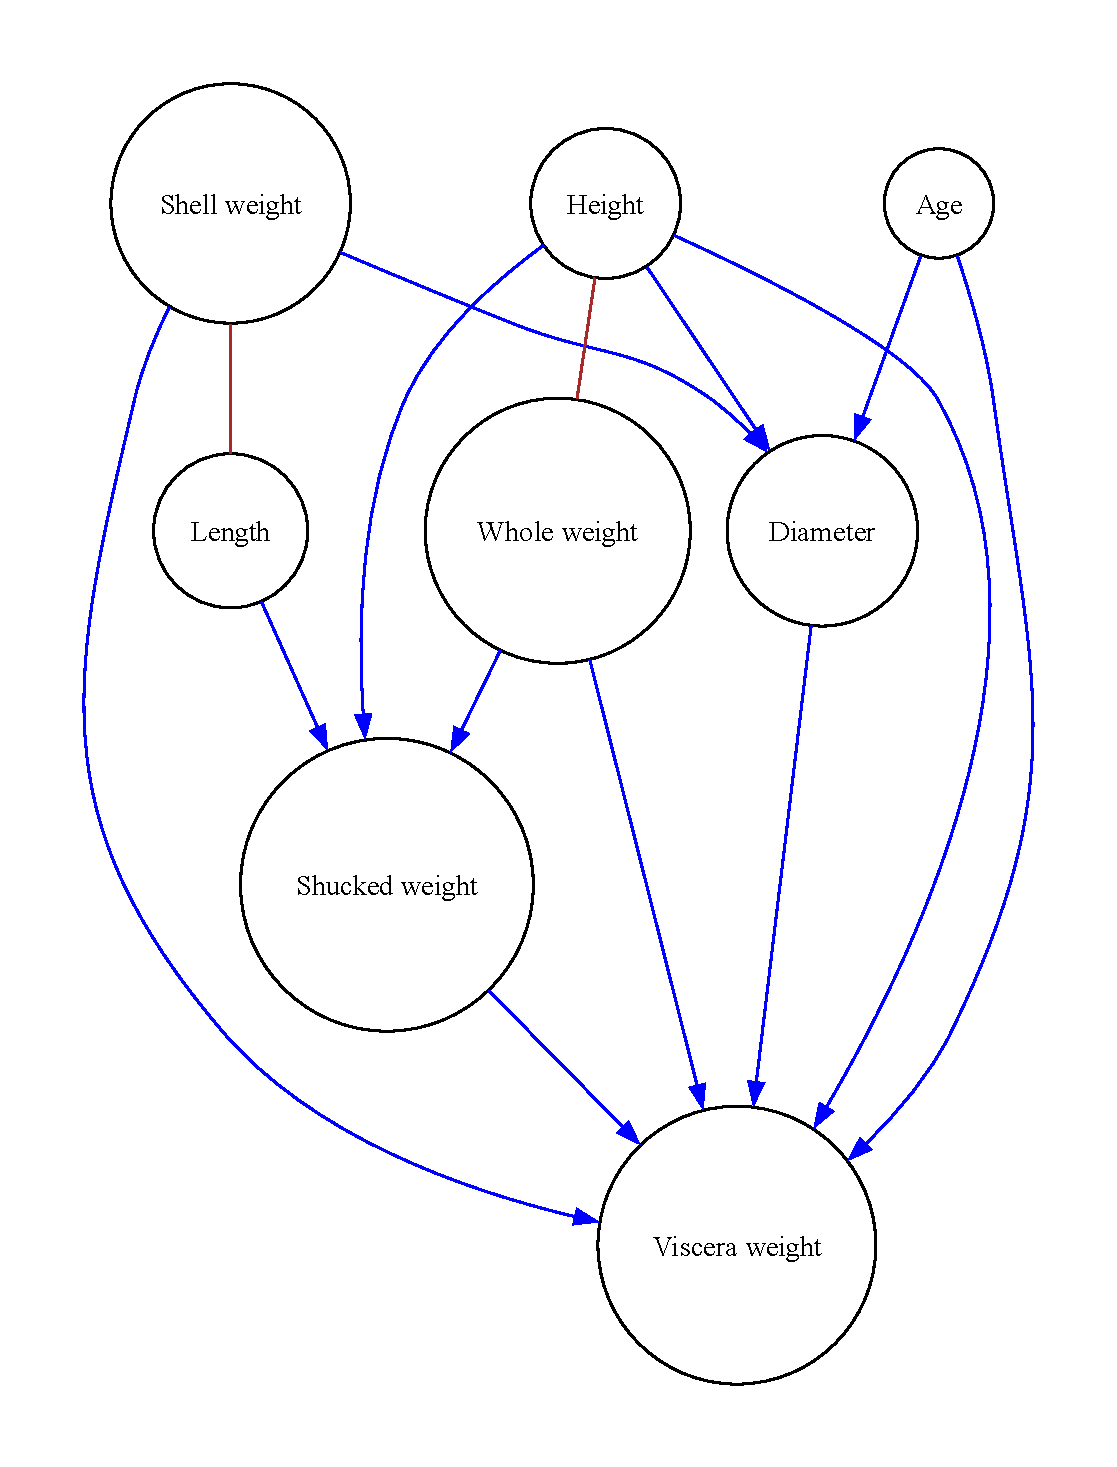
\includegraphics[height=0.4\textheight]{./demo_data/20241104_114158/Abalone/output_graph/initial_graph.pdf}
    \caption{Initial Graph}
\end{figure}

The above is the initial result graph produced by our algorithm.

The causal relationships among the various biological measurements indicate a complex interaction influenced by the developmental stage of the organism. Age plays a pivotal role as it impacts Diameter and Viscera weight, suggesting that as the organism matures, both the size and internal weight increase, reflecting its growth and development. Length influences both Shell weight and Shucked weight, indicating that longer organisms tend to have heavier shells and more substantial meat content. Additionally, Shell weight has a reciprocal influence on Length and is associated with Diameter and Viscera weight, highlighting how the physical characteristics of the shell and internal components are interconnected in terms of growth. Height also plays a significant role, affecting both Diameter and Whole weight along with Shucked and Viscera weights, which implies that as an organism becomes taller, there are cascading effects on its overall mass and internal structures. Ultimately, the interaction of these variables illustrates a growth-based hierarchy where age and physical measurements mutually reinforce each other in determining the organism's overall development.

\subsection{Revised Graph}
\begin{minipage}[t]{0.6\linewidth}
    By using the method mentioned in Section 4.4, we provide a revised graph pruned with Bootstrap and LLM suggestion. Pruning results are as follows.

    Bootstrap doesn't force or forbid any edges.
    
    The following are force results given by LLM:
    
    \begin{itemize}
        \item \textbf{Age $\rightarrow$ Length}: As abalones age, they generally grow larger; thus, age is a direct influencing factor on length.
        \item \textbf{Age $\rightarrow$ Shell weight}: Older abalones tend to have heavier shells because growth over time contributes to shell mass.
        \item \textbf{Age $\rightarrow$ Height}: The height of abalones typically increases with age, indicating a causal relationship between age and height.
        \item \textbf{Age $\rightarrow$ Whole weight}: Age affects the overall growth of abalones, which directly impacts their total weight, making age a causal factor for whole weight.
        \item \textbf{Age $\rightarrow$ Shucked weight}: As abalones grow older, they produce more edible flesh, which affects the shucked weight, establishing a causal link.
        \item \textbf{Length $\rightarrow$ Diameter}: Length and diameter are interrelated measures of size; as the length increases, it is reasonable to assume the diameter would increase as well.
        \item \textbf{Length $\rightarrow$ Height}: Similar to diameter, height is expected to rise as length increases, reflecting the growth pattern of abalones.
        \item \textbf{Length $\rightarrow$ Whole weight}: Longer abalones will naturally weigh more, establishing a causal relationship between length and whole weight.
        \item \textbf{Length $\rightarrow$ Viscera weight}: As abalones grow in length, their internal mass, including viscera, tends to increase, thereby causally linking length with viscera weight.
        \item \textbf{Shell weight $\rightarrow$ Height}: The shell weight contributes to the physical characteristics of the abalone, and its increase is usually associated with greater height.
        \item \textbf{Shell weight $\rightarrow$ Whole weight}: Shell weight is a component of the whole weight, thus it causally influences the total weight of the abalone.
        \item \textbf{Shell weight $\rightarrow$ Shucked weight}: The shucked weight represents the edible portion, which is influenced by the shell weight since larger shells can correlate with more flesh.
        \item \textbf{Diameter $\rightarrow$ Whole weight}: Diameter is a measure of size, and increasing the diameter of the abalone typically contributes to an increase in whole weight.
        \item \textbf{Diameter $\rightarrow$ Shucked weight}: Similarly, as the diameter increases, this is often associated with larger meat content, thereby affecting shucked weight.
    \end{itemize}
    
    The following are directions of remaining undirected edges determined by the LLM:
    \begin{itemize}
        \item \textbf{Length $\rightarrow$ Shell weight}: As abalones grow longer, their shells must also grow to support their increased size, leading to a causal relationship where longer abalones are likely to have heavier shells.
        \item \textbf{Height $\rightarrow$ Whole weight}: The height of an abalone contributes to its overall volume and mass; therefore, an increase in height is expected to result in an increase in whole weight as it directly affects the amount of flesh and shell present.
    \end{itemize}
    
    This structured approach ensures a comprehensive and methodical analysis of the causal relationships within the dataset.
\end{minipage}
\hfill
\begin{minipage}[t]{0.4\linewidth}
    \begin{figure}[H]
        \centering
        \vspace{-0.5cm}
        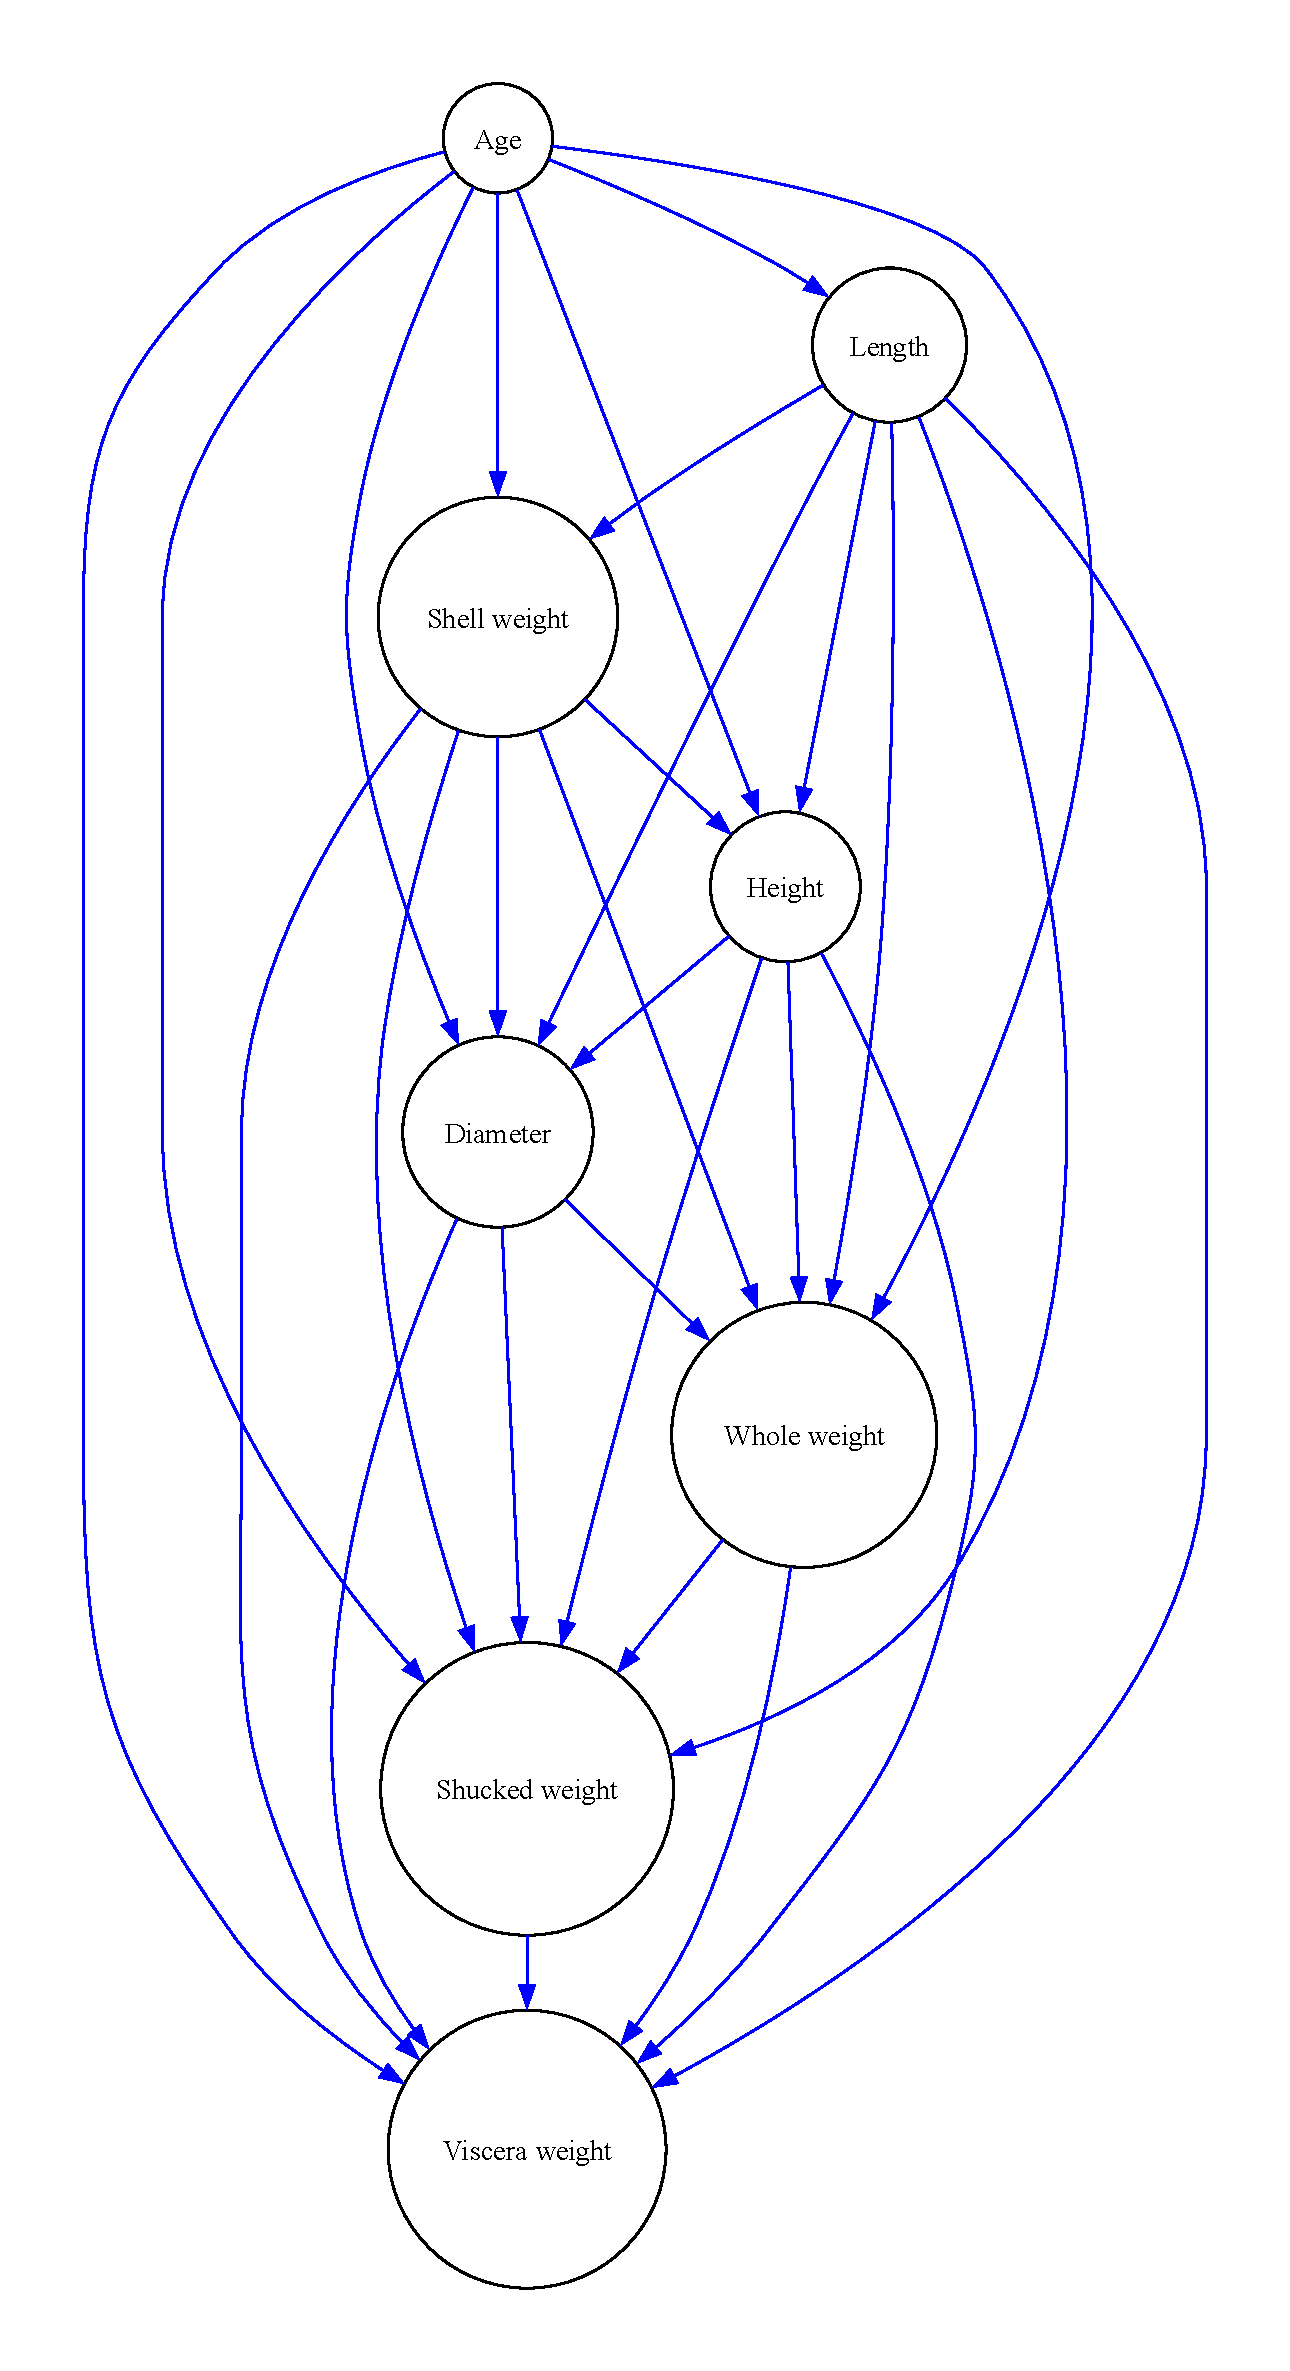
\includegraphics[width=\linewidth]{./demo_data/20241104_114158/Abalone/output_graph/revised_graph.pdf}
        \caption{\label{fig:corr}Revised Graph}
    \end{figure}
\end{minipage}

\subsection{Graph Reliability Analysis}
\begin{figure}[H]
    \centering
    \begin{subfigure}{0.32\textwidth}
        \centering
        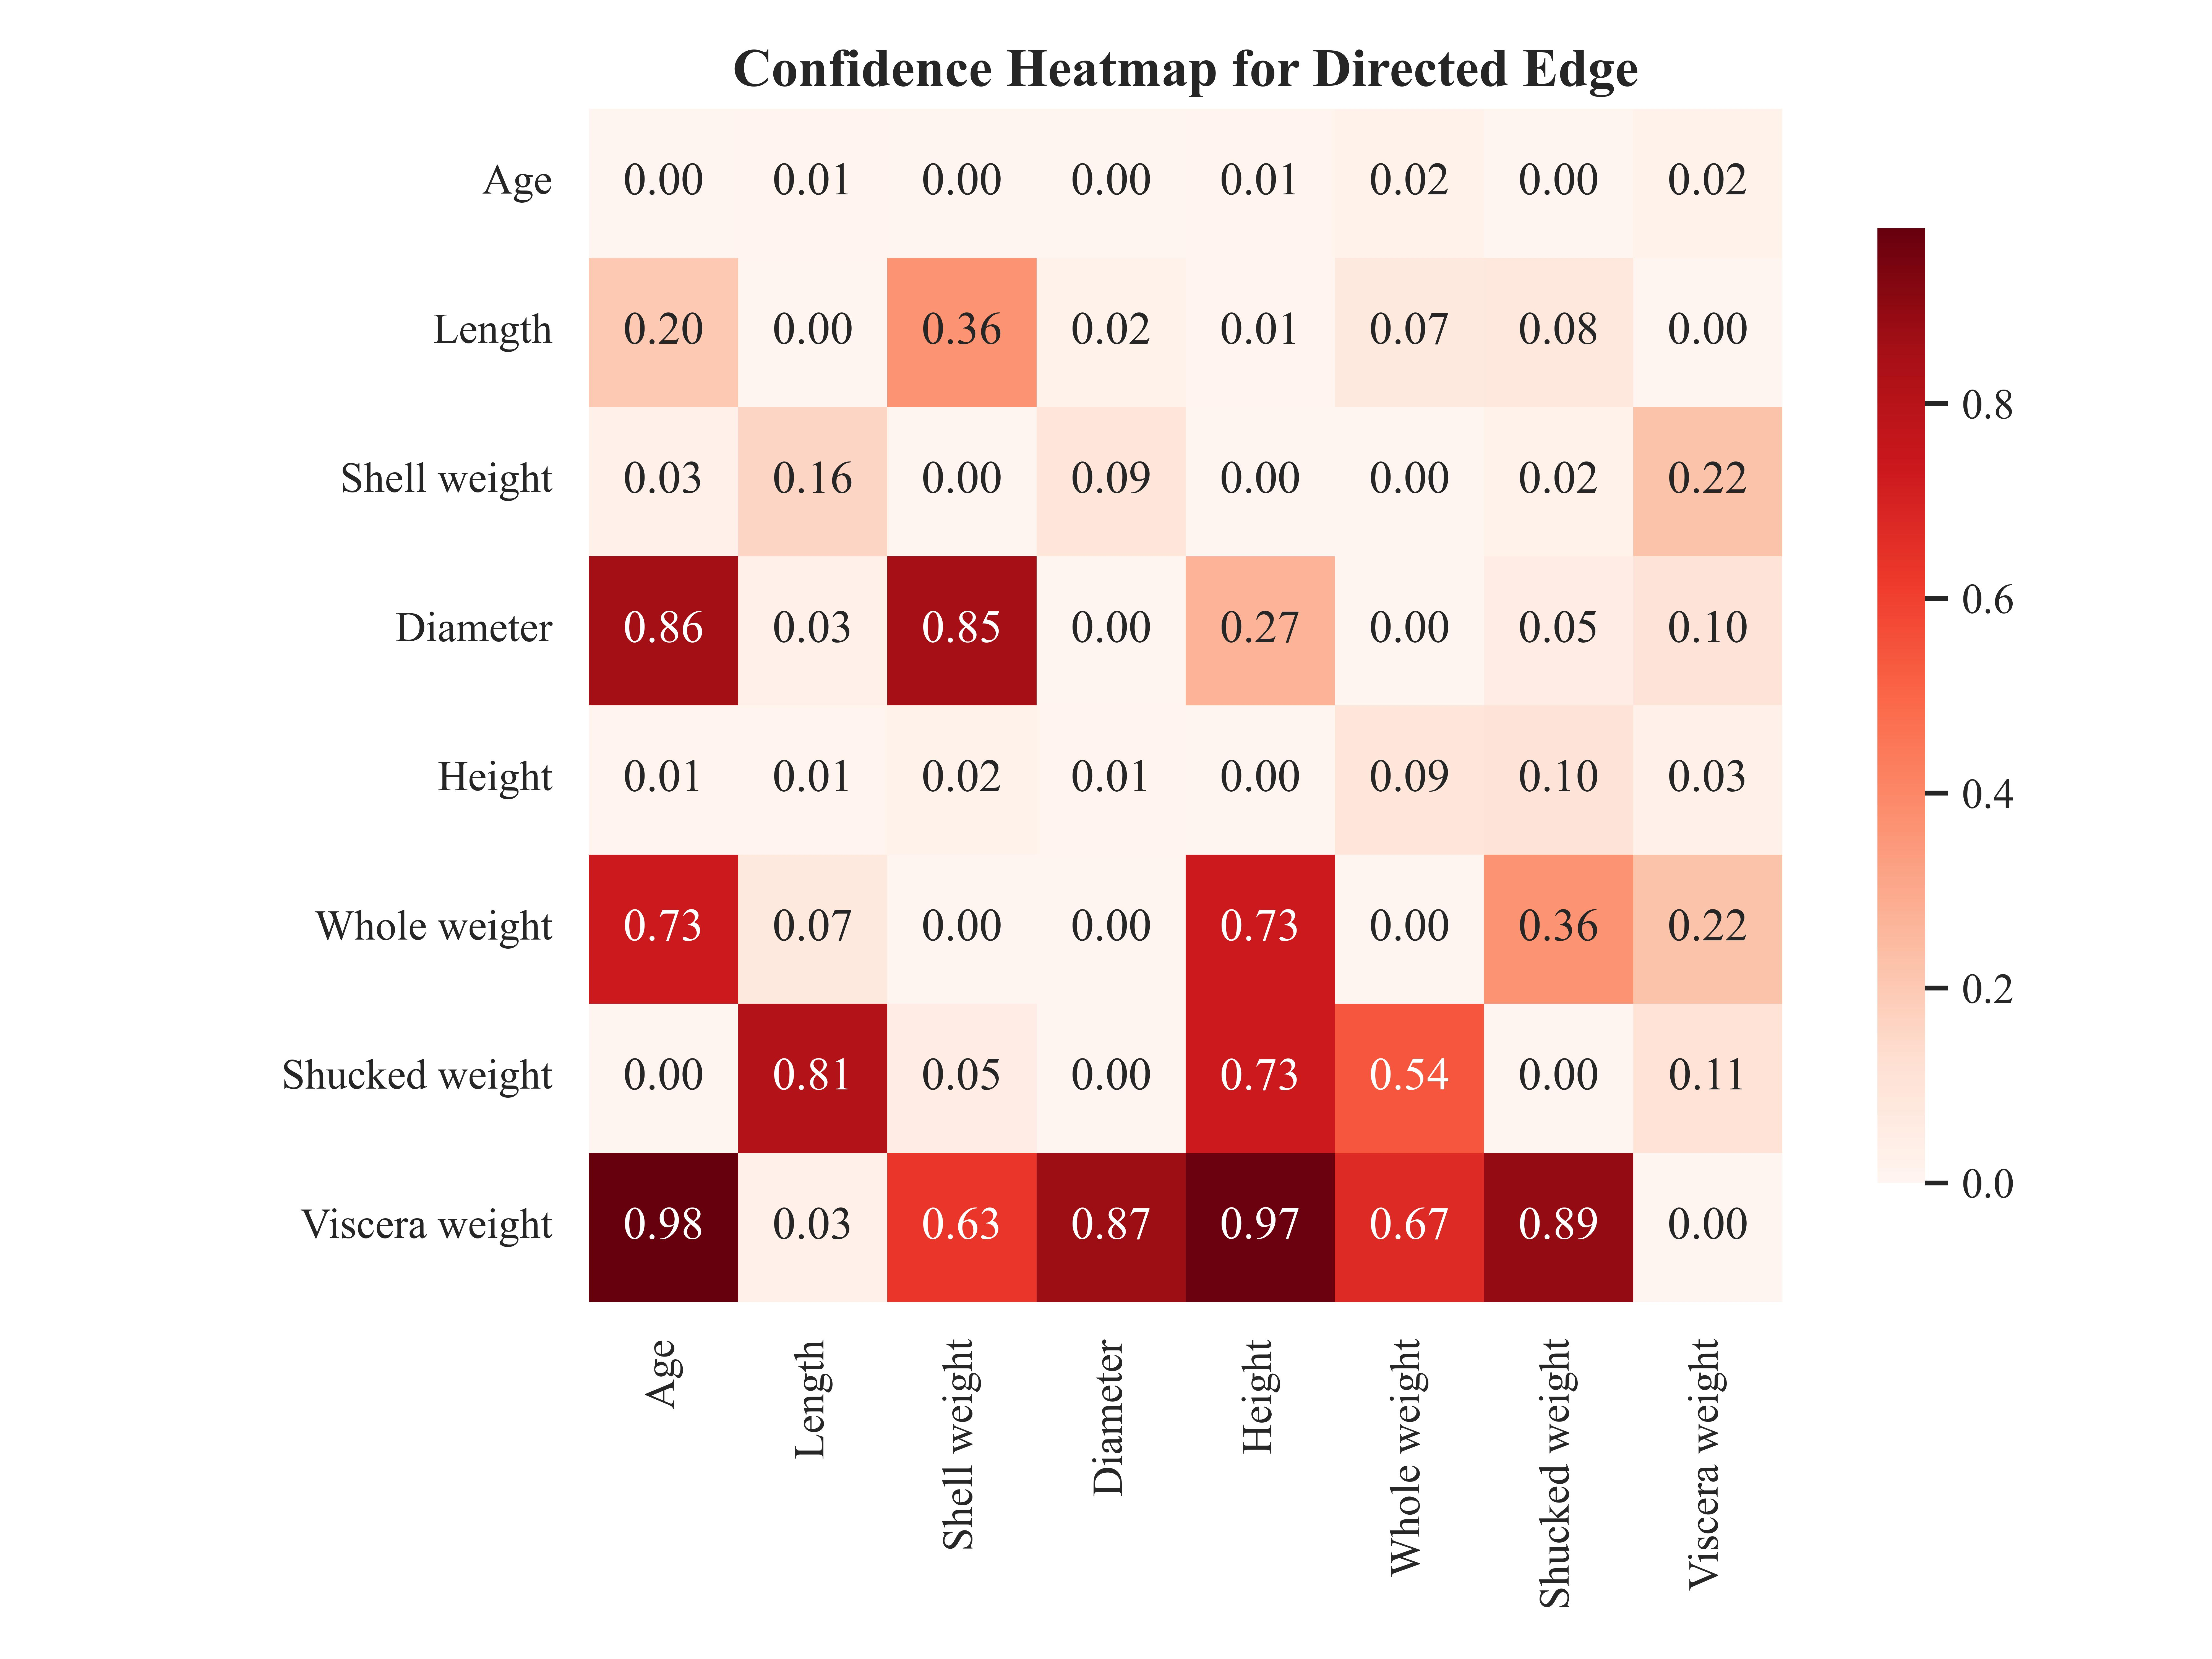
\includegraphics[width=\linewidth]{./demo_data/20241104_114158/Abalone/output_graph/certain_edges_confidence_heatmap.jpg}
        \caption{Directed Edge}
    \end{subfigure}
    \begin{subfigure}{0.32\textwidth}
        \centering
        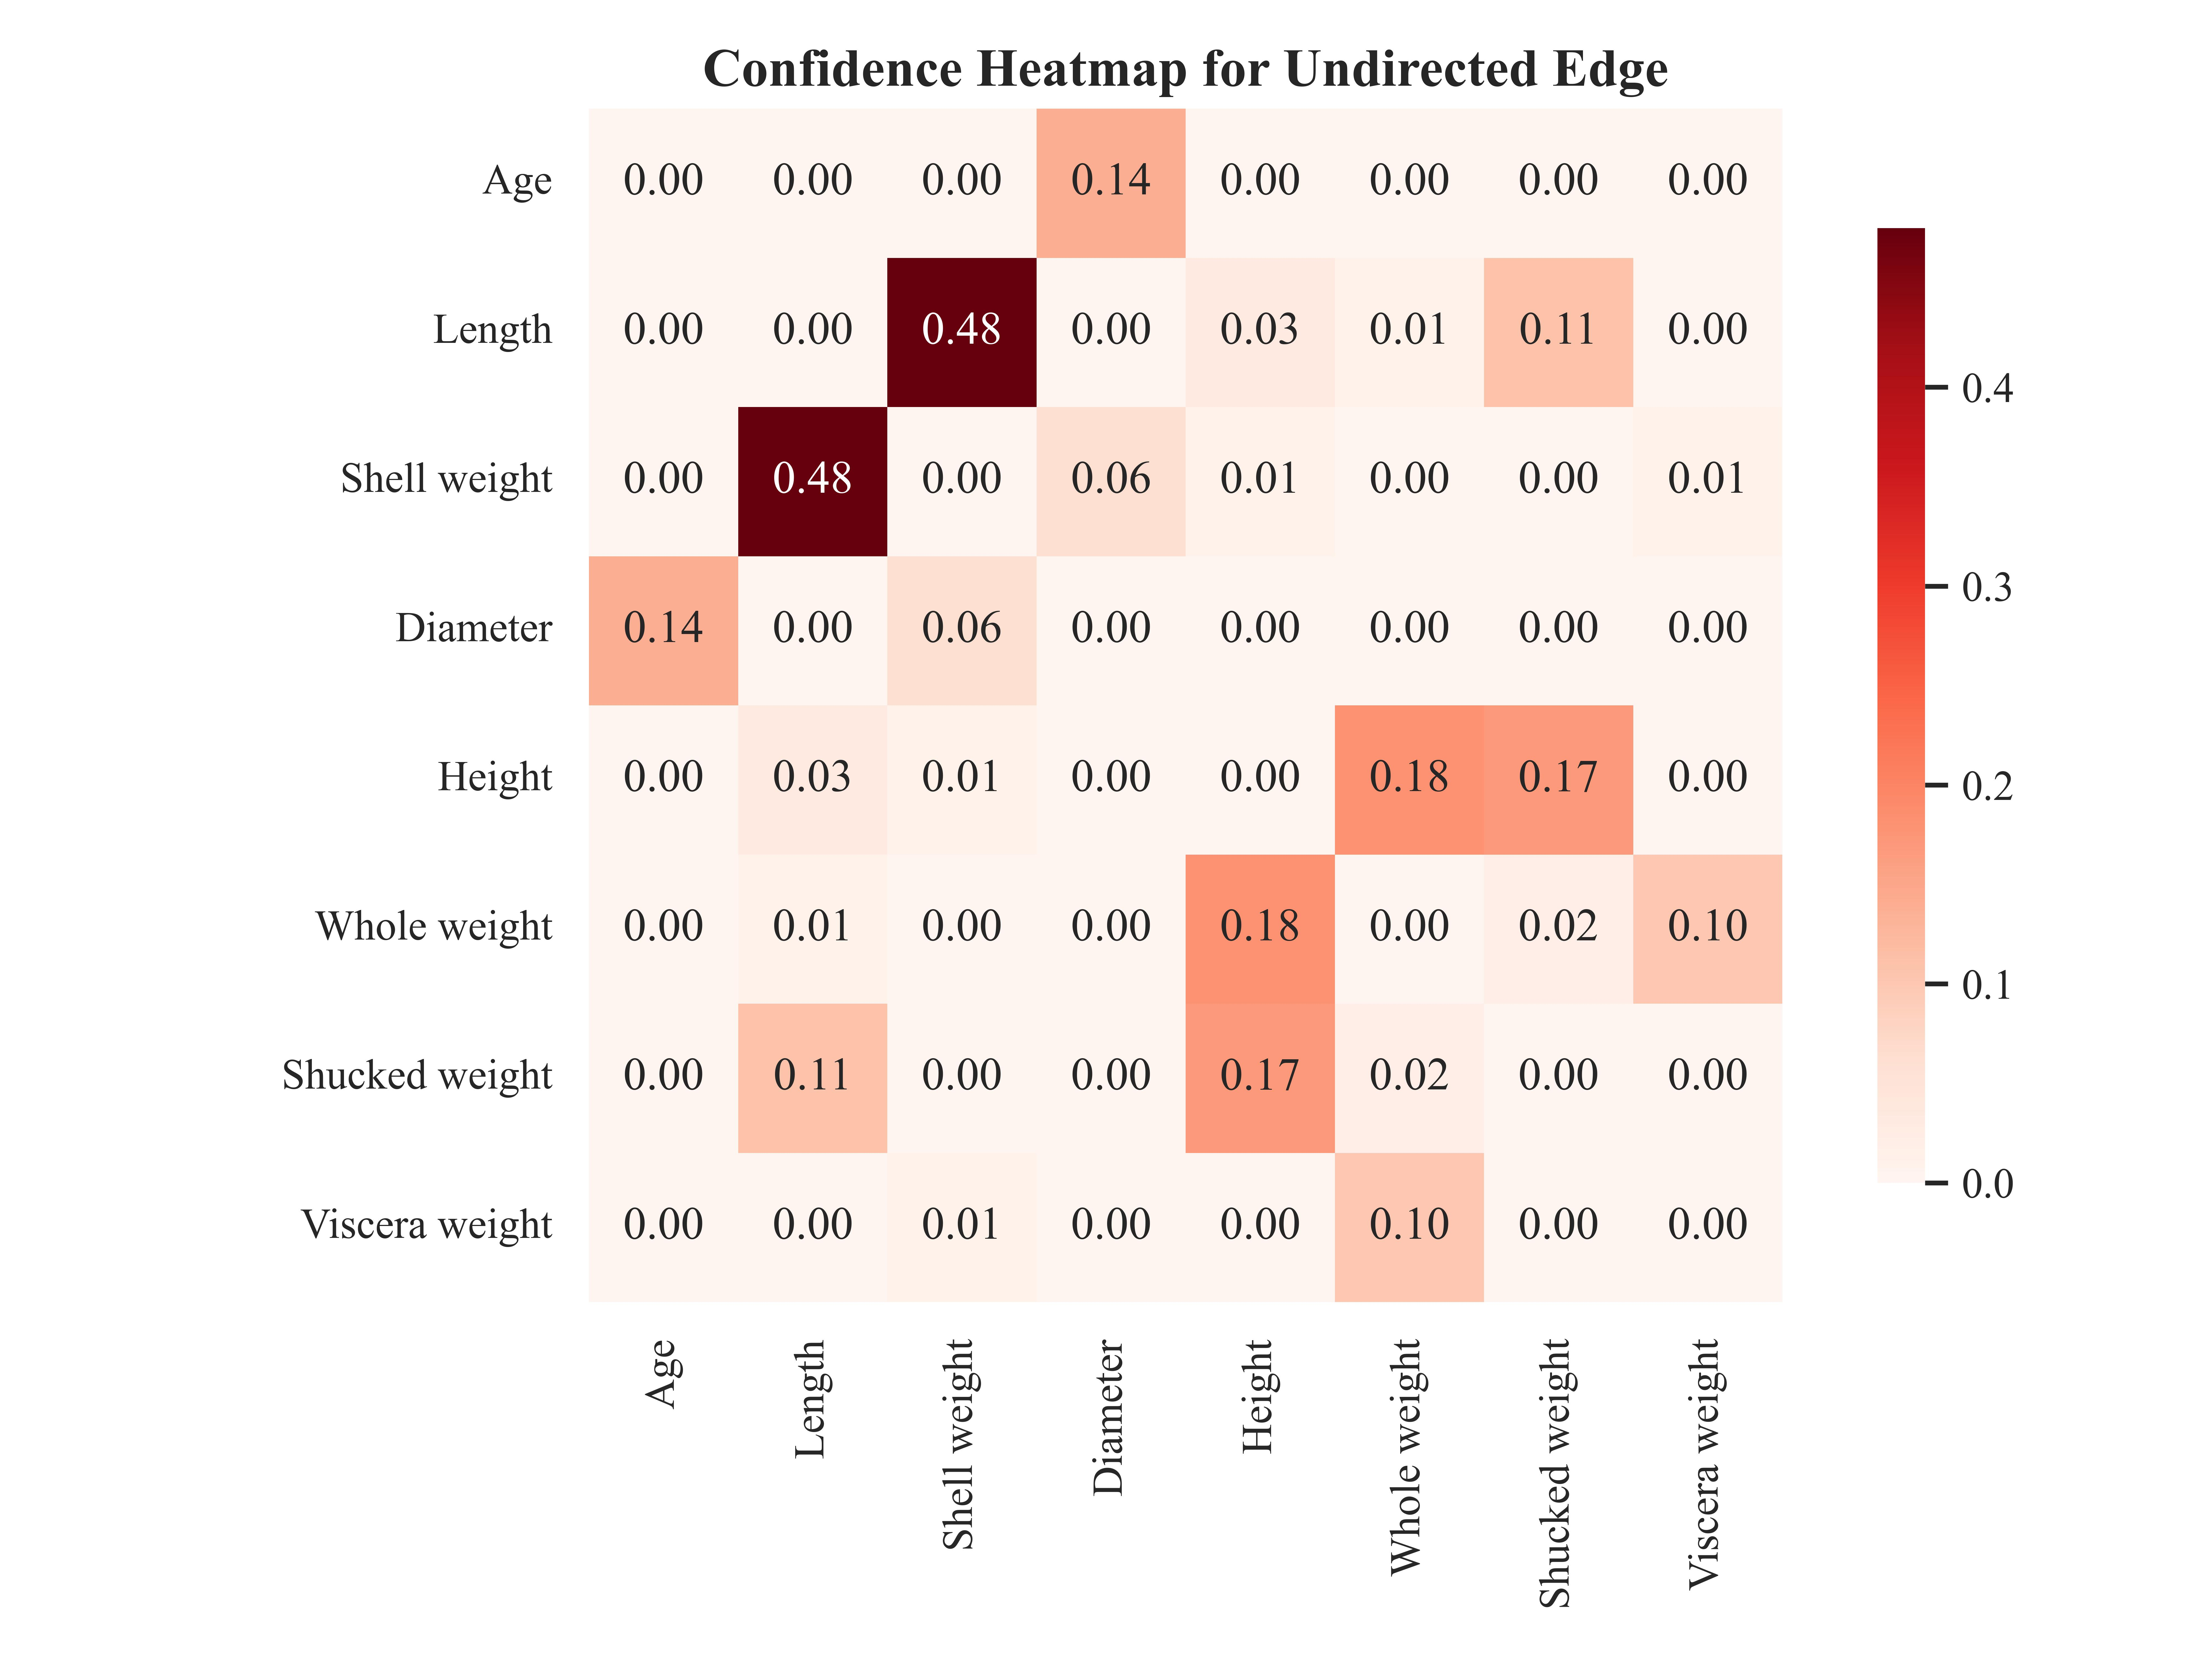
\includegraphics[width=\linewidth]{./demo_data/20241104_114158/Abalone/output_graph/uncertain_edges_confidence_heatmap.jpg}
        \caption{Undirected Edge}
    \end{subfigure}
    \begin{subfigure}{0.32\textwidth}
        \centering
        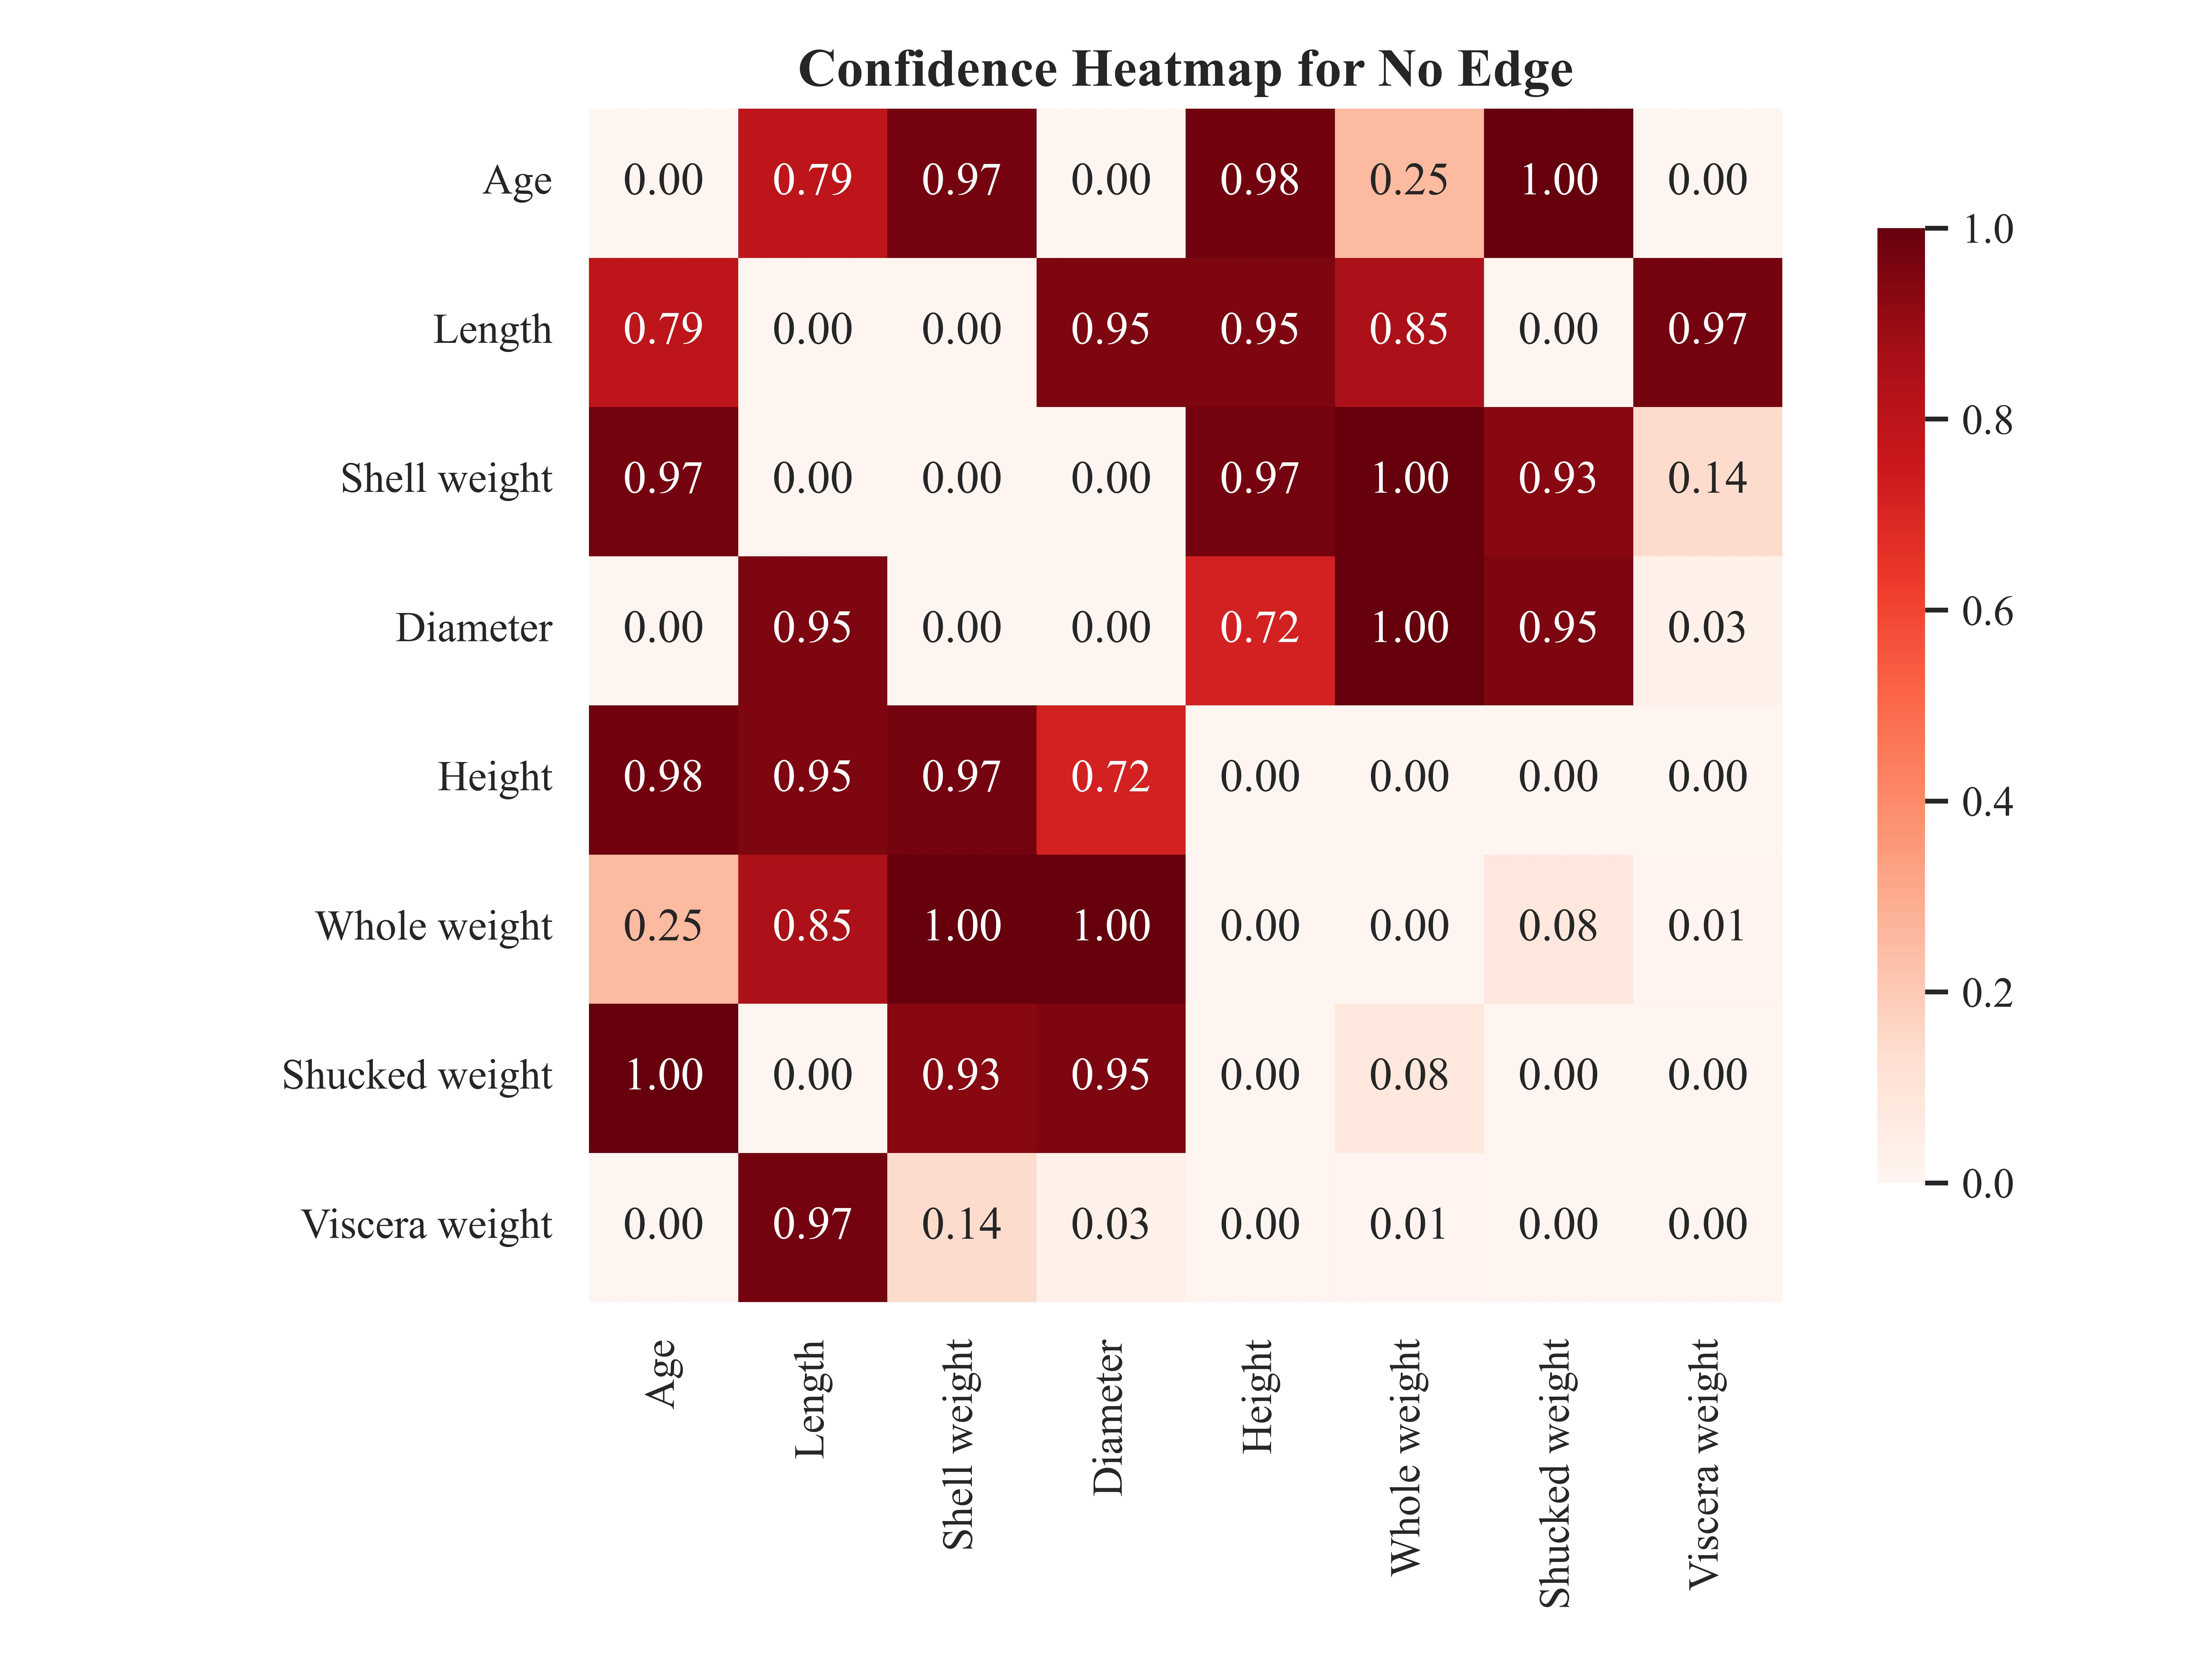
\includegraphics[width=\linewidth]{./demo_data/20241104_114158/Abalone/output_graph/non_existence_confidence_heatmap.jpg}
        \caption{No Edge}
    \end{subfigure}
    \caption{Confidence Heatmap of Different Edges}
\end{figure}        

The above heatmaps show the confidence probability we have on different kinds of edges, including directed edge ($\rightarrow$), undirected edge ($-$), No Edge, and probability of no edge. The heatmap of bi-edges is not shown because probabilities of all edges are 0. Based on the confidence probability heatmap and background knowledge, we can analyze the reliability of our graph.

From the statistical perspective, we have high confidence to believe that the edges connecting Whole Weight to Height (bootstrap probability of 0.73), Whole Weight to Shucked Weight (0.36), and Length to Shell Weight (0.36) exist, as these probabilities indicate a significant supportive relationship. Conversely, we have low confidence that the edges Age to Diameter (0.0), Age to Viscera Weight (0.02), and Height to Diameter (0.01) exist, suggesting that these relationships are statistically doubtful.

However, based on expert knowledge, we know that Age likely influences Length, Diameter, and Height significantly as abalones grow; thus, edges from Age to these measurements can be reasonably inferred to exist despite low statistical support. Moreover, the interdependencies among Length, Diameter, Height, and Whole Weight are also strongly supported by biological growth patterns, implying the existence of these causal connections. However, the low bootstrap probabilities of some edges imply caution, particularly regarding Age’s influence on Viscera Weight and Diameter.

Therefore, the result of this causal graph is partially reliable but should be interpreted with caution. Some edges are well-supported, while others, especially those with low bootstrap probability, may require further investigation to enhance our understanding of abalone growth dynamics.

\end{document}